\documentclass[12pt]{scrbook}

\usepackage{mdframed}
\usepackage{anyfontsize}
\usepackage{adjustbox}
\usepackage{graphicx}

% \newcommand{\orlymedia}{\includegraphics[scale=.08]{images/orly.png} {\Large\sffamily ORLY}}
\newcommand{\sbsmedia}{{\Large\sffamily Story Byte Studios}}



\mdfdefinestyle{l3style}{%
leftmargin=0pt,
backgroundcolor=black,
fontcolor=white,
linewidth=0pt,
innertopmargin=20pt,
innerbottommargin=20pt,
innerleftmargin=20pt,
font={\fontsize{50}{40}\selectfont}
}

\begin{document}

\pagestyle{empty}


\vspace{5em}

\begin{flushleft}
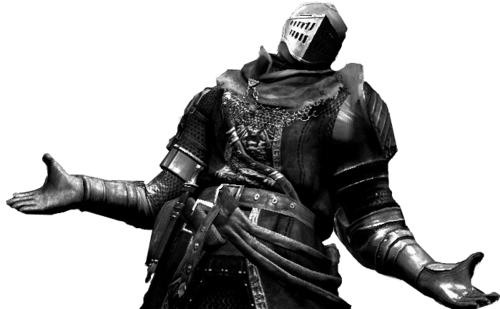
\includegraphics[scale=.88]{images/darkknight.png}
\end{flushleft}



%\vspace{-2.5em}

{\noindent\Large\emph{Programming}}\vspace{-0.3em}

\begin{mdframed}[style=l3style]
Role-Playing Games \par
\hspace{-.2cm}in Python
\end{mdframed}

\vspace{1em}


\begin{adjustbox}{minipage=.3\textwidth,right}
\Large\em
Geert-Jan Kruijff
\end{adjustbox}

\vfill

\sbsmedia

\tableofcontents 


% Introduction to the book
% Started: Wed 3 Oct 2018 


\chapter{Introduction} 

\section{Creating Adventures} 




\section{For Whom Is This Book?}


\section{Getting Things Set Up} 




\subsection{Mac} 

\subsection{Windows} 


\section{Conventions Used in This Book}


\section{Code Examples}

\section{Using Code Examples}

\section{Contacting the Author}



\end{document}